\originalchapter{22.02 2012 年期中卷}
题源: 2012年3月21日 Mid-Term Exam. 本章据对应官方答案重编并复算. 共有五道一级题, 首题包含八组短问.
\begin{exercise}\label{ex:2202-e2012-1}
原题 1. (a) 结合能主项正比 A 对核力意味着什么, 同 $A(A-1)$ 有何不同? (b) 判断: 聚变 Q 总为很大正值; Coulomb 排斥使聚变困难; 必须始终以 E>$V_C$ 才能聚变. (c) 可观测量定义、数学对象、例子. (d) 完备对易集是什么、为何需要; $\{L_{xy},L_z\}$, $L_{xy}=L_x^2+L_y^2$ 是否是? (e) 先测 $V(\hat x)$ 再测 x, 后者是否随机? (f) 态 $|-1,0\rangle$, $|0,-1\rangle$, $|1,0\rangle_z$, $|1,-1\rangle_y$ 哪些合法? (g) 深 $V_w$、宽2a有限阱, 偶能量态 E 是否束缚? (h) 一态为动量本征态, 另一为 H 本征态, 哪个是定态, 为什么?
\end{exercise}
\begin{solution}
(a) 核力短程、近邻饱和; 若所有粒子同等强耦合则对数目常按成对数 $A(A-1)/2$ 增长. (b) 第一不是对任意核种的普遍命题; 第二对带电核的低能聚变一般成立; 第三不成立, 隧穿允许 E低于势垒. (c) 自伴算符, 如 $p=-\ii\hbar\partial_x$. (d) 一组两两对易且联合标签足以区分态的算符. $[L_{xy},L_z]=0$, 因 $L_{xy}=L^2-L_z^2$, 在固定轨道角态空间与 $\{L^2,L_z\}$ 等价; 若包括径向、内禀自旋等自由度则还不完备. (e) 对易不保证测量后 x 确定: 非单射势如 $V=x^2$ 给同一 V 对应两个位置, 后测 x仍可能随机. 若 V 单调且非简并才可确定 x. (f) 前两个非法, 后两个合法. (g) 偶宇称本身不能决定, 需 E<0且正规可积, 或 E相对无穷远阈值低. (h) H本征态必是定态; 动量本征态只在 H与该态相容, 如自由粒子时也可能是定态, 一般有空间势时不能保证.
\end{solution}
\begin{exercise}\label{ex:2202-e2012-2}
原题 2. 一维经典热力学温度模型 $T=m\langle v^2\rangle/k_B$. (a) 用所学算符定义相应量. (b) 无限阱 $0<x<L$ 中每粒子态为
$\psi=\sqrt{1/(2L)}\sin(3\pi x/L)+\sqrt{1/L}\sin(10\pi x/L)+\sqrt{1/(2L)}\sin(11\pi x/L)$, 不做积分求其平均温度.
\end{exercise}
\begin{solution}
(a) 题设动能代理算符 $\hat T=\hat p^2/(mk_B)=2H_{\rm kin}/k_B$. 它不是一般纯态独立定义出的热力学温度, 这里只按等分配模型比较动能. (b) 归一阱态系数为 $1/2,1/\sqrt2,1/2$, 能量概率为 $1/4,1/2,1/4$. 所以 $\langle T\rangle=\hbar^2\pi^2[9/4+100/2+121/4]/(mk_BL^2)=82.5\hbar^2\pi^2/(mk_BL^2)$. 无须积分因 H已对角.
\end{solution}
\begin{exercise}\label{ex:2202-e2012-3}
原题 3. 一维中子源通量 $\Phi_{\rm inc}$、能量E, 保护墙厚L建模为 $V>E$ 方势垒, 后方探测器测通量. (a) 画模型和波形特点. (b) 小透射极限下测得多少通量?
\end{exercise}
\begin{solution}
左侧是入射和反射叠加, 墙内指数波, 右侧只有同波长的低幅透射. $\kappa=\sqrt{2m_n(V-E)}/\hbar$, 测得 $\Phi_{\rm det}=T\Phi_{\rm inc}$, 厚垒 $T\simeq16E(V-E)V^{-2}\e^{-2\kappa L}$. 若只要求指数精度, 可写 $O(1)\e^{-2\kappa L}$, 不把前因子4当作任何 E/V 的精确常数. 这是课程一维势模型; 真实中子屏蔽包括碰撞、吸收和能谱输运, 不能用单粒子方垒替代工程屏蔽计算.
\begin{center}\begin{tikzpicture}[x=1cm,y=.65cm]
\draw[->](-3,0)--(4,0)node[right]{$x$};\draw[->](-3,0)--(-3,3)node[above]{$V,\operatorname{Re}\psi$};
\draw[thick](-3,0)--(0,0)--(0,2.5)--(1.7,2.5)--(1.7,0)--(4,0);
\draw[dashed](-3,1.6)--(4,1.6)node[right]{$E<V$};
\draw[structurecolor,thick,domain=-3:0,samples=80]plot(\x,{.9*cos(180*\x)});
\draw[structurecolor,thick,domain=0:1.7,samples=50]plot(\x,{.9*exp(-2.2*\x)});
\draw[structurecolor,thick,domain=1.7:4,samples=80]plot(\x,{.022*cos(180*(\x-1.7))});
\node[below]at(-1.5,-1){入射与反射叠加};\node[below]at(.85,-1){指数区};\node[below]at(2.8,-1){小幅透射};
\draw[<->](0,2.9)--(1.7,2.9)node[midway,above]{$L$};
\end{tikzpicture}\end{center}
图仅显示振荡、指数和透射幅度的定性关系, 各段示意曲线不用于读取匹配常数; 精确复波函数应同时匹配函数与导数.

\end{solution}
\begin{exercise}\label{ex:2202-e2012-4}
原题 4. $^{250}_{96}$Cm 质量232.938 GeV. 设两体裂变为 $^{130}_{52}$Te (121.002 GeV) 与 $^{120}_{44}$Ru (111.724 GeV), 无伴随中子. 取 $\hbar c=197$ MeV fm、$e^2/(\hbar c)=1/137$, $r_0=1.25$ fm. (a) 预计稳定吗? (b) Q, 同 alpha 比较. (c) 接触 $R=R_{\rm Te}+R_{\rm Ru}$ 的 Coulomb 势、转折点 $R_c$. (d) 约化质量, 方垒高度 $V_H=V_C(R)$、宽 $R_c-R$ 的 T. (e) 核阱深35 MeV, 相对动能按 Q+35, 求 f=v/R. (f) 衰变率及半衰期. 源题明确此两体裂变模型非常粗糙, 真实裂变有碎片分布和中子.
\end{exercise}
\begin{solution}
(a) 重且中子过多, 预计放射性不稳定. (b) 由给定口径质量 Q=$212$ MeV, 比典型 alpha 的数MeV大得多. (c) $R=12.498$ fm, $C=52\cdot44\cdot197/137=3290.04$ MeV fm, $V_C=263.25$ MeV, $R_c=C/Q=15.519$ fm. (d) $\mu c^2=121002\cdot111724/(121002+111724)=58089.0$ MeV, L=3.0213 fm, $\kappa=12.386$ fm$^{-1}$. 用完整厚垒前因子得 $T\simeq7.84\times10^{-33}$. (e) $v/c=\sqrt{2(212+35)/58089}=0.0922$, $f\simeq2.214\times10^{21}$ s$^{-1}$. (f) $\lambda=fT\simeq1.74\times10^{-11}$ s$^{-1}$, $t_{1/2}\simeq3.99\times10^{10}$ s, 约1266年. 采用仅指数或不同前因子会显著改变该粗估, 原题质量舍入也极敏感. 不把此值当作 Cm 实测半衰期, 更不忽略原题关于真实多体裂变的警告.
\end{solution}
\begin{exercise}\label{ex:2202-e2012-5}
原题 5。图中A--C为三幅分段势及各自的绿色能线，1--7为所画波函数实部。逐条判断1--7能否作为图A、B或C中能量$E$的定态；可同时对应多幅图，也可均不对应。用边界连续性、允许区波长、禁阻区形状和散射边界条件说明。
\end{exercise}
\begin{center}
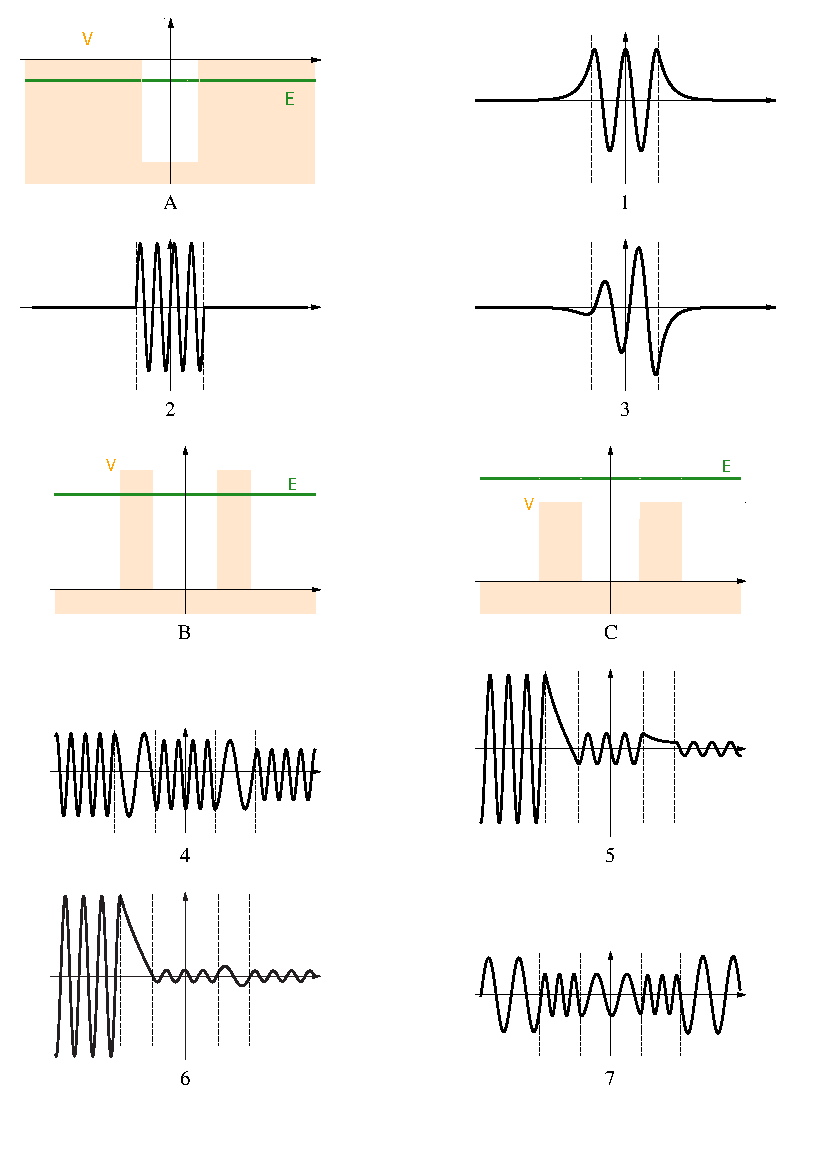
\includegraphics[width=.80\linewidth]{figures/ocw-exam-2012-q5.pdf}\\
{\small 原题图：Paola Cappellaro，MIT 22.02 Spring 2012 OCW，2012期中题卷第3页，裁取矢量图。}
\end{center}
\begin{solution}
官方源图定性配对 A--1, B--5, C--4. 曲线2与有限势边界的函数及导数连续性不符, 更像硬墙模型但仍须核对端点条件. 曲线3在一维对称有限井的非简并束缚能级中不是定态; 偶奇叠加一般涉及不同能量. 曲线6需要两个高度不同的势垒, E低于第一个而高于第二个, 不对应B. 曲线7在中央区动能更大、波长更短, 需要势井而非图C的势垒. 每个允许区的波长由 E-V 决定, 禁阻区指数是否增长还依散射方向与有限区匹配. 此题源图没有数值标尺, 判定针对上述特征, 不以采样曲线冒充严格 Schrödinger 解.
\end{solution}
